\section{Traversals}
\label{sec:traversals}

\begin{frame}
	\frametitle{Tree traversals}
	\framesubtitle{Walking through our tree}

	\begin{center}
		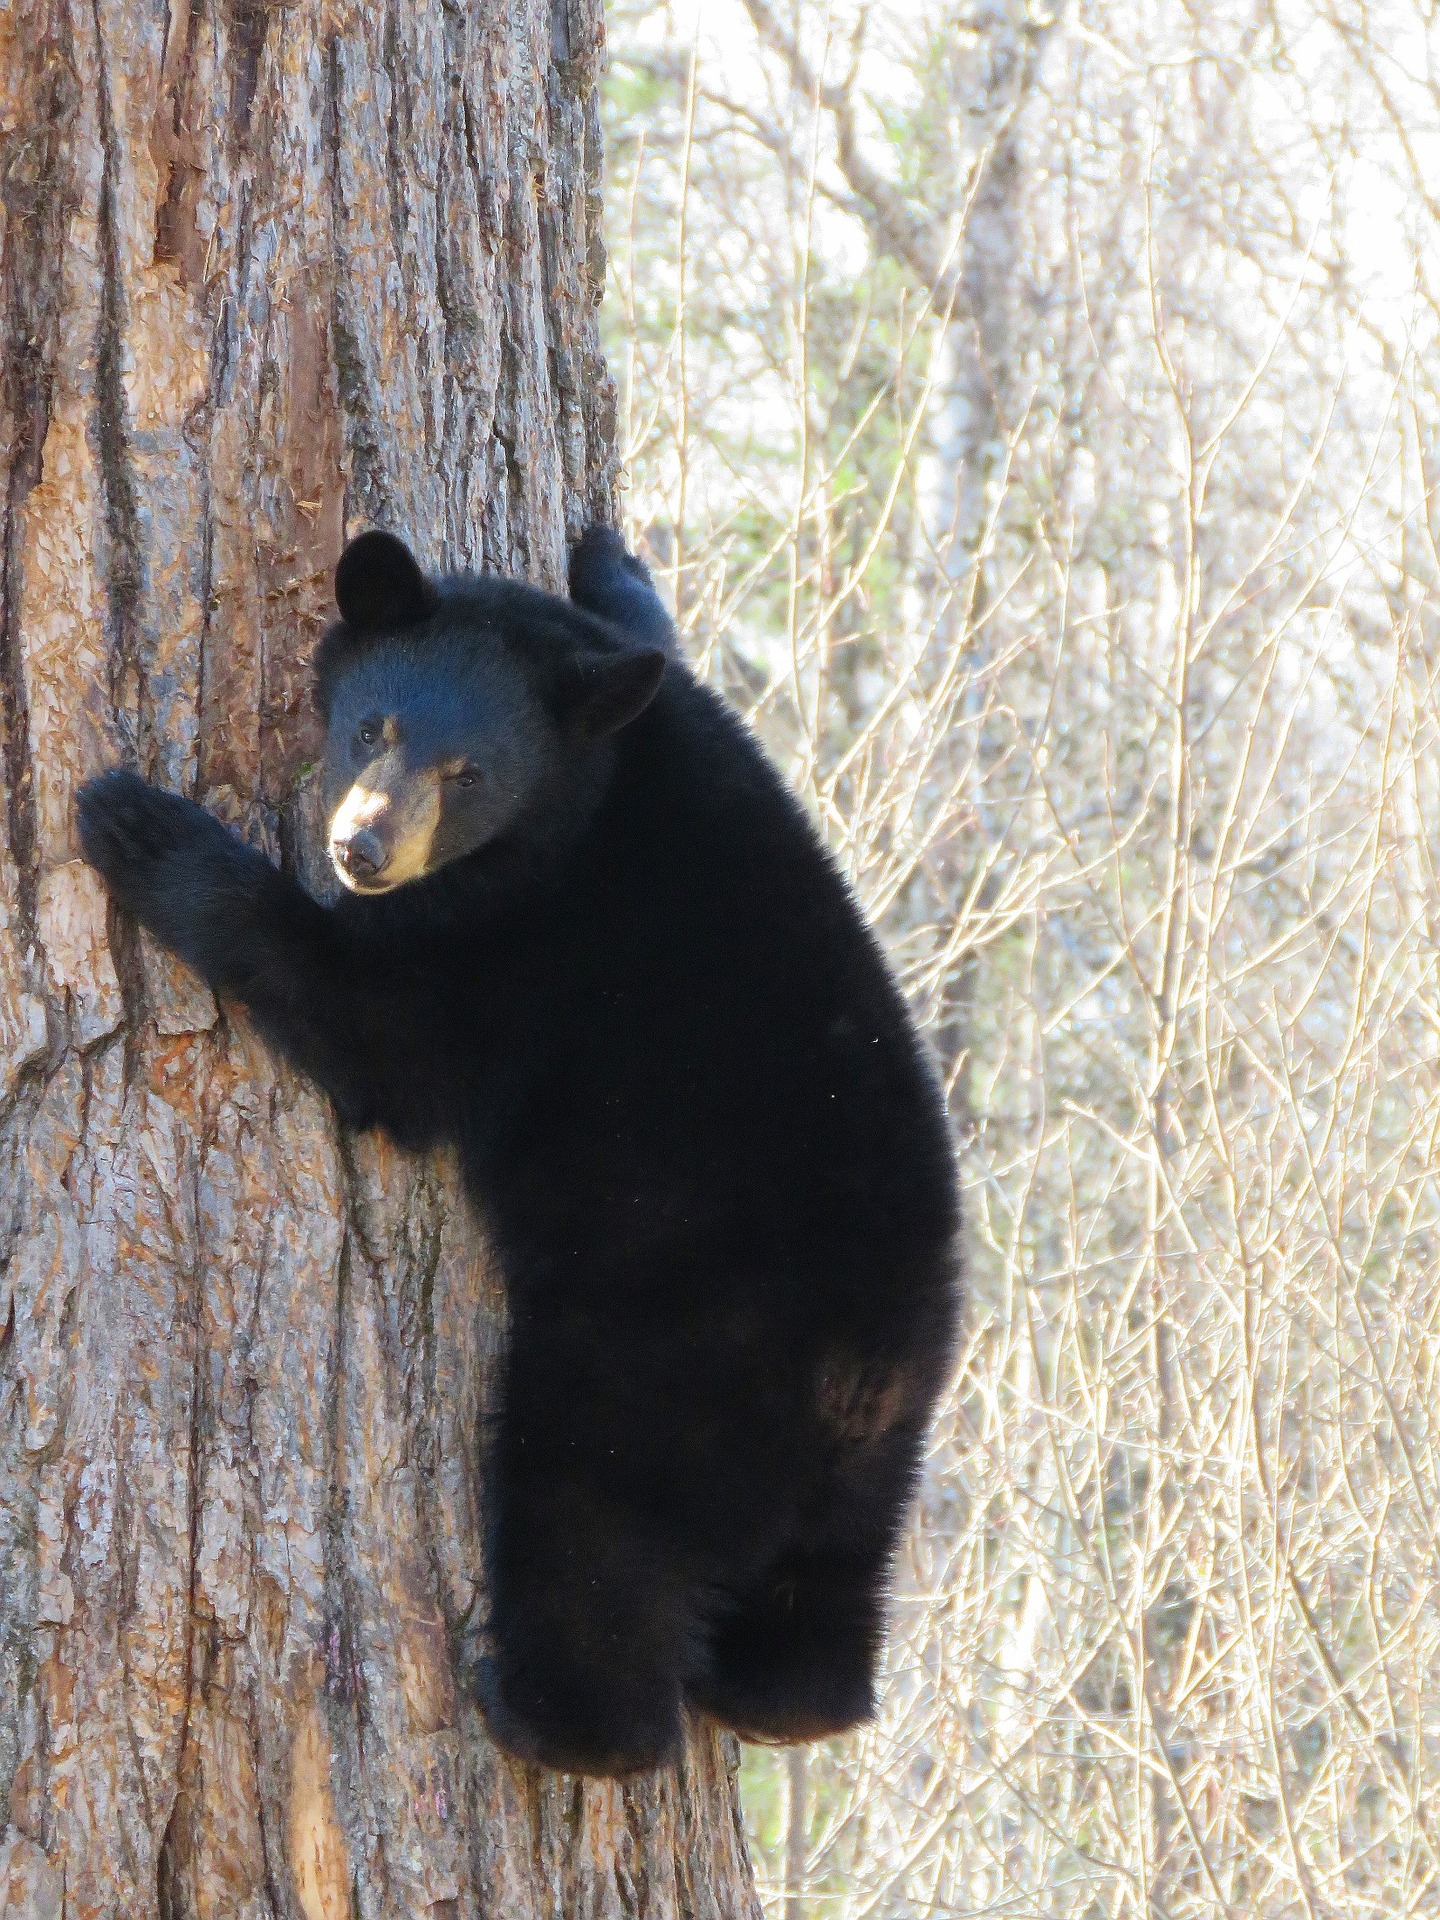
\includegraphics[trim={0 4cm 0 4cm},clip, width=0.65\textwidth]{figures/bearcub.jpg}\\
		\hspace*{15pt}\hbox{\scriptsize Image By:\thinspace{\itshape Skeeze}}
		% https://pixabay.com/photos/bear-cub-brown-climbing-tree-1576559/
	\end{center}

\end{frame}

\begin{frame}
	\frametitle{Iterating over the nodes}
	
		\begin{block}{Finding all the nodes}
			If you want to iterate over the tree, you can do so in many different orders. Three common ones for binary trees are:
			\begin{itemize}
				\item Pre-order traversal
				\item In-order traversal
				\item Post-order traversal
			\end{itemize}
		\end{block}	
\end{frame}

\begin{frame}
	\frametitle{Pre-order traversal}
	\begin{overlayarea}{\textwidth}{\textheight}
			\begin{columns}
				\column{0.455\textwidth}
				\begin{itemize}
					\item First give the value of the current node.
					\item Then a pre-order traversal of the left child.
					\item Then a pre-order traversal of the right child.
				\end{itemize}
				\column{0.455\textwidth}
				\pause
					\begin{tikzpicture}[
						level distance = 2.5em,
						level 1/.style={sibling distance=9em},
						level 2/.style={sibling distance=4.5em},
						level 3/.style={sibling distance=2.25em},
					]
					\node[ellipse,onslide=<3>{draw=red}] (t1) {\alert<3>{1}}
					child { node[ellipse,onslide=<4>{draw=red}]   {\alert<4>{2}}
						child { node[ellipse,onslide=<5>{draw=red}] {\alert<5>{3}}}
						}
						child { node[ellipse,onslide=<6>{draw=red}]   {\alert<6>{4}}
							child { node[ellipse,onslide=<7>{draw=red}] {\alert<7>{5}}}
							child { node[ellipse,onslide=<8>{draw=red}] {\alert<8>{6}}
								child { node[ellipse,onslide=<9>{draw=red}] {\alert<9>{7}}}
								child { node[ellipse,onslide=<10>{draw=red}] {\alert<10>{8}}}
							}
						};
					\end{tikzpicture}
			\end{columns}
			\only<11>{
			\begin{exampleblock}{Amsterdam, Rotterdam, no not that kind of topology!}
				Gives us a \textit{topological} order of the tree.\\
				If all nodes represent jobs, and job $i$ depends on it's parent job $p$ then this gives us an order in which we can
				do all jobs, satisfying these dependencies.
			\end{exampleblock}
		}
	\end{overlayarea}
\end{frame}

\begin{frame}
	\frametitle{In-order traversal}
	\begin{overlayarea}{\textwidth}{\textheight}
			\begin{columns}
				\column{0.455\textwidth}
				\begin{itemize}
					\item First an in-order traversal of the left child.
					\item Then give the value of the current node.
					\item Then an in-order traversal of the right child.
				\end{itemize}
				\column{0.455\textwidth}
					\begin{tikzpicture}[
						level distance = 2.5em,
						level 1/.style={sibling distance=9em},
						level 2/.style={sibling distance=4.5em},
						level 3/.style={sibling distance=2.25em},
					]
					\node[ellipse,onslide=<5>{draw=red}] (t1) {\alert<5>{1}}
					child { node[ellipse,onslide=<4>{draw=red}]   {\alert<4>{2}}
						child { node[ellipse,onslide=<3>{draw=red}] {\alert<3>{3}}}
						}
						child { node[ellipse,onslide=<7>{draw=red}]   {\alert<7>{4}}
							child { node[ellipse,onslide=<6>{draw=red}] {\alert<6>{5}}}
							child { node[ellipse,onslide=<9>{draw=red}] {\alert<9>{6}}
								child { node[ellipse,onslide=<8>{draw=red}] {\alert<8>{7}}}
								child { node[ellipse,onslide=<10>{draw=red}] {\alert<10>{8}}}
							}
						};
					\end{tikzpicture}
			\end{columns}
			\only<2>{
				\begin{questionblock}{In-order}
				What is the order of nodes now?
				\begin{multicols}{2}
					\begin{enumerate}[A.]
						\item 1,2,3,4,5,6,7,8
						\item 3,2,1,5,4,7,6,8
						\item 3,2,8,7,6,5,4,1
						\item 8,7,6,5,4,3,2,1
					\end{enumerate}
				\end{multicols}
			\end{questionblock}
		}
			\only<11>{
				\begin{exampleblock}{We'll save that for tomorrow}
				We will see an example for this tomrrow!
			\end{exampleblock}
		}
	\end{overlayarea}
\end{frame}

\begin{frame}
	\frametitle{Post-order traversal}
	\begin{overlayarea}{\textwidth}{\textheight}
			\begin{columns}
				\column{0.455\textwidth}
				\begin{itemize}
					\item First a post-order traversal of the left child.
					\item Then a post-order traversal of the right child.
					\item Then give the value of the current node.
				\end{itemize}
				\column{0.455\textwidth}
					\begin{tikzpicture}[
						level distance = 2.5em,
						level 1/.style={sibling distance=9em},
						level 2/.style={sibling distance=4.5em},
						level 3/.style={sibling distance=2.25em},
					]
					\node[ellipse,onslide=<10>{draw=red}] (t1) {\alert<10>{1}}
					child { node[ellipse,onslide=<4>{draw=red}]   {\alert<4>{2}}
						child { node[ellipse,onslide=<3>{draw=red}] {\alert<3>{3}}}
						}
						child { node[ellipse,onslide=<9>{draw=red}]   {\alert<9>{4}}
							child { node[ellipse,onslide=<5>{draw=red}] {\alert<5>{5}}}
							child { node[ellipse,onslide=<8>{draw=red}] {\alert<8>{6}}
								child { node[ellipse,onslide=<6>{draw=red}] {\alert<6>{7}}}
								child { node[ellipse,onslide=<7>{draw=red}] {\alert<7>{8}}}
							}
						};
					\end{tikzpicture}
			\end{columns}
			\only<2>{
				\begin{questionblock}{Post-order}
				What is the order of nodes now?
				\begin{multicols}{2}
					\begin{enumerate}[A.]
						\item 1,2,3,4,5,6,7,8
						\item 3,2,5,8,7,6,4,1
						\item 3,2,8,7,6,5,4,1
						\item 8,7,6,5,4,3,2,1
					\end{enumerate}
				\end{multicols}
			\end{questionblock}
		}
			\only<11>{
				\begin{exampleblock}{I didn't mean to sound so dark :(}
				Used to delete a tree (first delete your children, before deleting yourself).
			\end{exampleblock}
		}
	\end{overlayarea}
\end{frame}
